\newcommand{\code}{\texttt}

\chapter{Introduction}
// TODO

\chapter{Platypus}
Moderné procesory od výrobcu \emph{intel} majú na svojich čipoch integrované obvody a čítače pre počítanie a ukladanie odhadu spotreby niektorých častí procesora.
Prístup k týmto čítačom (sekcia \ref{sec:rapl}) bol pôvodne neprivilegovaný, čo otváralo možnosti potenciálnych postranných útokov, a na základe čoho bola rodina útokov
Platypus vyvinutá. Jedná sa o plne softvérové útoky, ktorými je možné extrahovať rôzne citlivé informácie z napadnutého systému. Medzi samotné útoky
patrí rozlišovanie vykonávaných inštrukcií, rozlišovanie veľkostí operandov inštrukcií, prípadne aj získanie RSA kľúča zo \emph{square-and-always-multiply} algoritmu.

\section{Intel RAPL} \label{sec:rapl}
Moderné \emph{intel} procesory poskytujú \emph{RAPL} (Running Average Power Limit) rozhrania pre monitorovanie odhadovanej akumulovanej spotreby procesora
od jeho resetu. Táto spotreba je ukladaná v modelu špecifických registroch (MSR) a je ju možné čítať priamo (rozhrania \code{/dev/msr} alebo \code{/dev/safe-msr}),
prípadne za pomoci rámca \code{powercap}. Týmto spôsobom meraná spotreba je často využívaná pre rôzne účely ako sú modulácia výkonu procesora,
sledovanie spotreby, prípadne profilovanie softvéru.

RAPL poskytuje údaje pre rôzne domény procesora:
\begin{itemize}
    \item \emph{core} pre konkrétne jadro procesora,
    \item \emph{uncore} pre integrované grafické čipy apod.,
    \item \emph{package} zahŕňajúci core a uncore domény,
    \item \emph{DRAM} pre systémovú pamäť pre daný soket.
\end{itemize}
Toto rozdelenie platí pre väčšinu procesorov, avšak niektoré nové procesory obsahujú viac, než jednu package doménu na jednom čipe, prípadne sa dopĺňa
nová doména \emph{psys}. % // TODO cituj/footnote https://github.com/powercap/powercap/issues/3
RAPL registre sa podľa zistení \cite{Platypus} aktualizujú raz za $1000 \mu s$ pre doménu package a DRAM a raz za $50 \mu s$ pre doménu core.
Rámec \code{powercap} umožňuje jednoduchý prístup k týmto doménam.

\section{Analýza výkonu}
V niektorých prípadoch je na hardvéri možné vykonávať postrannú analýzu systému fyzicky. Takéto prístupy vyžadujú špeciálne pomôcky,
ktoré majú vysokú vzorkovaciu frekvenciu, vďaka čomu je často možné získať dostatočné množstvo dát o systéme v rámci jednej alebo
iba niekoľkých \emph{stôp}\footnote{Stopa (angl. trace) je množina hodnôt získaných počas analýzy.}.
Takáto analýza sa nazýva \emph{SPA} (angl. Simple Power Analysis) a pre účely tejto práce nie je vhodná.

Typ analýzy \emph{DPA} (angl. Differential Power Analysis) využíva veľké množstvo získaných stôp, na ktorých je vykonaná štatistická analýza.
Výhodou tejto metódy je schopnosť spriemerovať šum, vďaka čomu sa môžu detegovať aj veľmi malé výchylky v spotrebe \cite{Platypus}. V niektrých prípadoch sú tieto
výchylky spôsobované napríklad operandami inštrukcií, ktoré nie sú pomocou SPA ľahko (alebo vôbec) detegovateľné. Prístup DPA je vhodný aj pre
prípady, keď je vzorkovacia frekvencia výrazne obmedzená.


\section{Základné súčasti experimentov}
// TODO ?
%Experimenty vykonávané v tejto práci majú niekoľko stavebných blokov.

\section{Experimenty}
Táto práca sa pokúsila reprodukovať niektoré časti publikácie \cite{Platypus}.
// TODO uvod do sekcie

Procesor, na ktorom boli vykonávané experimenty je \emph{Intel Core i5-4200U CPU @ 1.60GHz}. Bola využitá knižnica
powercap\footnote{Knižnica powercap \href{https://github.com/powercap/powercap}{https://github.com/powercap/powercap}.} pre čítanie RAPL registrov
a implementácia rozhrania pre čítanie TSC (Time Stamp Counter) registra\footnote{Rozhranie pre čítanie TSC registra\\\href{https://github.com/LITMUS-RT/liblitmus/blob/master/arch/x86/include/asm/cycles.h}{https://github.com/LITMUS-RT/liblitmus/blob/master/arch/x86/include/asm/cycles.h}.}.

\subsection{Analýza spotreby energie pre jednotlivé inštrukcie}
Spotreba energie inštrukcií bola meraná pomocou RAPL rozhrania, čo znamená, že vzorkovacia frekvencia je prinízka pre meranie spotreby jedného spustenia inštrukcie.
Ako kompenzácia pre túto skutočnosť sa každá inštrukcia spúšťala $50000$-krát po sebe a bola zmeraná celková spotreba od začiatku behu po koniec. Tieto spustenia
boli zabalené do cyklu, čím sa ale pridala nežiadaná réžia do merania. Vplyv na spotrebu energie tejto réžie bol odstránený odpočítaním zmeranej spotreby
prázdneho cyklu od získaných meraní pre inštrukciu. Spotreba bola takto pre každú inštrukciu meraná toľkokrát, kým sa nezískalo $10000$ nenulových stôp.
Ošetrenie pre prijatie iba nenulovej stopy je z dôvodu, že pri mnohých inštrukciách, ktorých rýchlosť vykonania je prinízka, sa RAPL čítače nestihnú aktualizovať.

Na obrázku \ref{img:instruction_comparison} je zobrazená energetická spotreba niekoľkých inštrukcií. Inštrukcie pre túto vizualizáciu boli zvolené rovnaké
ako v \cite{Platypus} pre možnosť porovnania rozdielnych vzťahov medzi spotrebami týchto inštrukcií.

\begin{figure}\label{img:instruction_comparison}
  \centering
  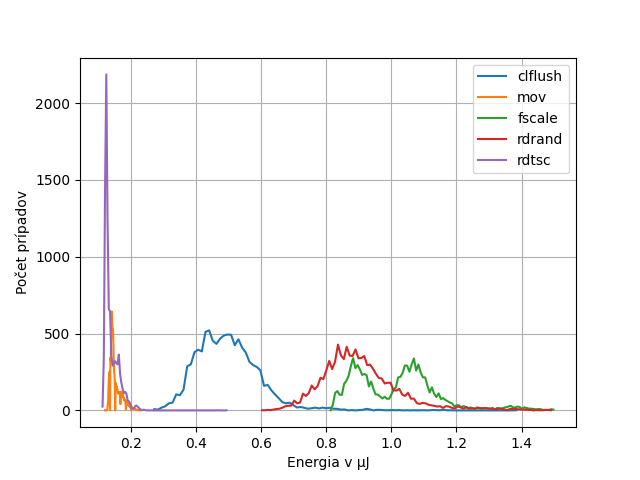
\includegraphics[scale=0.7]{./obrazky-figures/instr_comparison.png}
  \caption{Porovnanie spotreby vybraných inštrukcií.}
\end{figure}

Základným predpokladom postranného útoku na zistenie vykonávaných inštrukcií je schopnosť rozlíšenia inštrukcií na základe ich spotreby.

